\documentclass[10pt]{exam}
\usepackage[hon]{template-for-exam}
\usepackage{tikz,multicol,cclicenses,hyperref,silence}
\usetikzlibrary{shadings,shadows,arrows.meta,shapes.geometric}
\footer{}{\thepage}{\sc \myclass}

\WarningFilter{latex}{Label `question}
\WarningFilter{latex}{Label `part}
\WarningFilter{latex}{There were multiply-defined labels}


\title{Rotational Motion Notes}
\author{Rohrbach}
\date{\today}

\begin{document}
\maketitle

\section*{Angular Quantities}
\subsection*{Measuring Angles}
\begin{tikzpicture}
  \draw[dotted] (0,3) -- (0,-3);
  \draw[dotted] (3,0) -- (-3,0);
  \draw[thin] circle (2);
  \path (2,0) coordinate (b);
  \draw[ultra thick, red] (b) arc (0:57.29:2)
    coordinate (e);
  \draw[dashed,red] (0,0) -- (e);
  \draw[dashed,red] (0,0) -- (b);
\end{tikzpicture}
%
\hfill
%
\begin{tikzpicture}[scale=0.7]
  \draw[dotted] (0,3) -- (0,-3);
  \draw[dotted] (3,0) -- (-3,0);
  \draw[thin] circle (2);
  \path (2,0) coordinate (b);
  \draw[ultra thick, blue] (b) arc (0:120:2)
    coordinate (e);
  \draw[dashed,blue] (0,0) -- (e);
  \draw[dashed,blue] (0,0) -- (b);
\end{tikzpicture}
\vs

\subsection*{Conversions}
\vs



\subsection*{Angular Kinematic Quantities}

\renewcommand{\arraystretch}{2}

\begin{tabular}{p{9em}ccp{6.5em}}
  Concept & Linear/Translational Quantity & Angular/Rotational Quantity & \hfill ``Bridge'' \\ \hline\hline
  position \\[2em]\hline
  displacement \\[1em] & units: & units:  \\\hline
  velocity \\[1em] & units: & units:  \\\hline
  acceleration \\[1em] & units: & units: \\\hline
\end{tabular}


\pagebreak


\section*{Practice}

\begin{questions}
  
% \question 
%   When you look at the Sun from the surface of the Earth, it subtends an angle of about 0.5$^\circ$ in the sky.  The Earth is 150 million km away from the Sun.  (a) Convert your angle to radians.  (b) Estimate the diameter of the Sun.

%   \begin{tikzpicture}
%     \draw[shading=ball] (0,0) circle (0.2);
%     \draw (2.5:10) -- (0,0) -- (-2.5:10);
%     \draw[->] (-2.5:4) arc (-2.5:2.5:4) 
%       node[midway,anchor=west] {$0.5^\circ$};
%     \fill[
%       shading=ball, 
%       ball color=orange,
%       circular glow={fill=yellow}, 
%       draw=yellow
%     ] 
%     (10,0) circle (.5);
%   \end{tikzpicture}

%   \vs

\question
  A bicycle has wheels of diameter 68 cm. If the bicycle travels 92 km, how many rotations do the wheels make?
  \vs


\question
  A wheel of radius 1.3 meters is accelerating at a rate of 12 rad/s$^2$. At the moment that the wheel is rotating at 3.2 rad/s,
  %
  \begin{parts}
    \part what is the magnitude of \emph{tangential} acceleration at a point on the outside of the wheel?
    \part what is the magnitude of \emph{radial} (centripetal) acceleration at a point on the outside of the wheel?
    \part what is the magnitude of the \emph{total} acceleration at a point on the outside of the wheel?
  \end{parts}
  \vs

\end{questions}

\pagebreak
%%%%%%%%%%%%%%%%%%%%%%%%%%%%%%%%%%%%%%%%

\section*{Rotational Kinematic Equations}

\begin{multicols}{3}
  \begin{center}
      \emph{``Old Faithful''} 
      %
      \begin{align*}
        v = v_0 + a t
      \end{align*}

      \columnbreak
      
      \emph{``The Big Chalupa''} 
      %
      \begin{align*}
        x = x_0 + v_0t + \frac{1}{2}at^2
      \end{align*}

      \columnbreak
      
      \emph{``Ain't Got No Time''}
      %
      \begin{align*}
        v^2 = v_0^2 + 2a \left( x - x_0 \right)
      \end{align*}

  \end{center}
\end{multicols}

\vspace{5em}

\subsection*{Practice}

Pilots can be tested for the stresses of flying high-speed jets in a whirling ``human centrifuge,'' which starts at rest and takes 1.0 min to turn through 20 complete revolutions before reaching its final speed.

\vspace{2em}

\begin{parts}
  \part 
    What was its angular acceleration (assumed constant)?
  \part
    What was its final angular speed {\bf in rpm}?
\end{parts}



\pagebreak \hfill \pagebreak
%%%%%%%%%%%%%%%%%%%%%%%%%%%%%%%%%%%%%%%%

\section*{Rotational Dynamics}

\subsection*{Quantities}

\renewcommand{\arraystretch}{2}

\begin{tabular}{p{9em}ccp{6.5em}}
  Concept & Linear/Translational Quantity & Angular/Rotational Quantity & \hfill ``Bridge'' \\ \hline\hline
  cause of acceleration \\[1em] & units: & units:  \\\hline
  inertia \\[1em] & units: & units:  \\\hline
\end{tabular}

\vs

\subsection*{Moment of Inertia for Extended Objects}

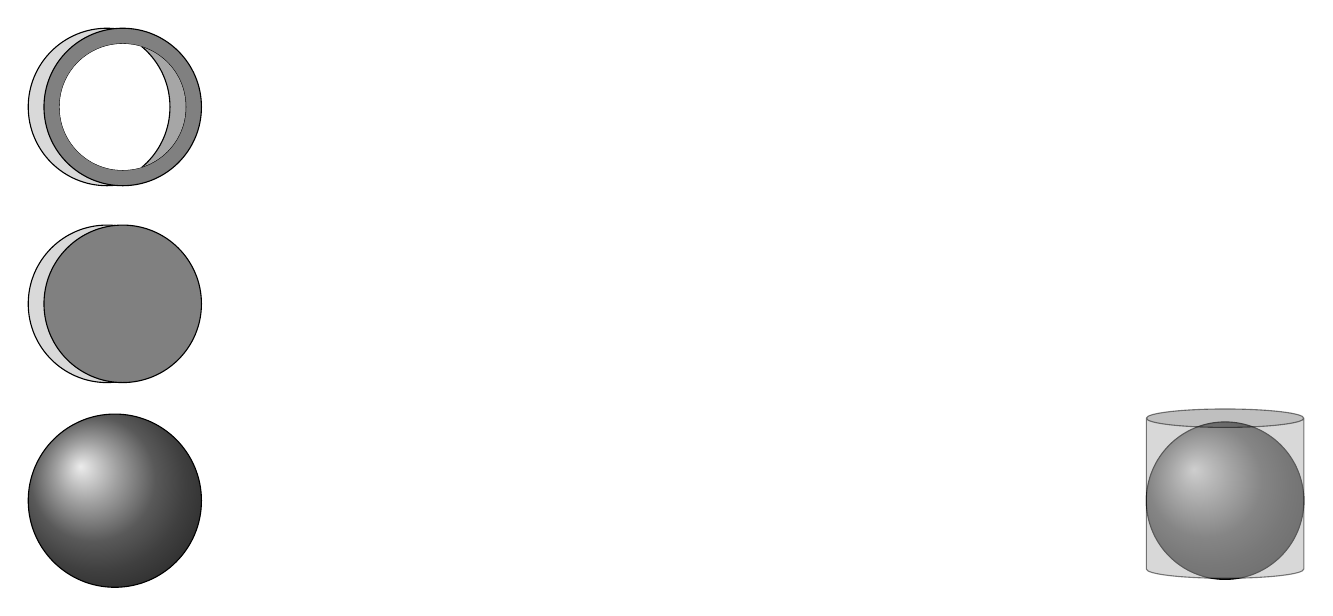
\begin{tikzpicture}
  % \begin{scope}
  %   \draw (0,0) circle (1) (0.1,0.1) circle (1);
  % \end{scope}

  \begin{scope}
    \draw[fill=gray!30] (-0.2,0) circle (1);
    \draw[fill=gray] (0,0) circle (1);
    \draw[fill=white] (0,0) circle (.8);

    \begin{scope}
      \clip (0,0) circle (.8);
      \draw (0,0) circle (.8);
      \fill[gray!70] (-1,-1) rectangle (1,1);
      \draw[fill=white] (-0.4,0) circle (1);
    \end{scope}

  \end{scope}

  % \begin{scope}[shift={(0,-2.5)}]
  %   \node[
  %       cylinder, 
  %       draw=black, 
  %       shape border rotate=90,
  %       minimum width=2cm,
  %       cylinder uses custom fill,
  %       cylinder body fill = gray!60,
  %       cylinder end fill = gray
  %       ] at (0,0) {};
  % \end{scope}

  \begin{scope}[shift={(0,-2.5)}]
    \draw[fill=gray!30] (-0.2,0) circle (1);
    \draw[fill=gray] (0,0) circle (1);
  \end{scope}

  \begin{scope}[shift={(0,-5)}]
    \draw[ball color=gray] (-0.1,0) circle (1.1);
  \end{scope}

  \begin{scope}[shift={(14,-5)}]

    \draw[ball color=gray] (0,0) circle (1);

    \node[
      cylinder, 
      draw=black, 
      semitransparent,
      shape border rotate=90,
      minimum size=2cm,
      minimum height=2.15cm,
      cylinder uses custom fill,
      cylinder body fill = gray!60,
      cylinder end fill = gray
      ] at (-0,0) {};

  \end{scope}
\end{tikzpicture}


\pagebreak

\subsection*{Practice}

\begin{questions}
  

\question
  Consider the following situation:


  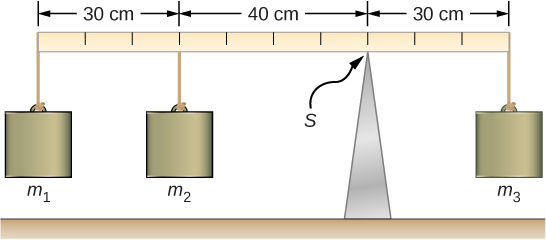
\includegraphics{torque_question.jpg}

  {\footnotesize Image Credit: OpenStax \emph{University Physics}. Authored by: OpenStax CNX. }

  {\footnotesize License:} \cc\hspace{-1em}\ccby  {\footnotesize CC BY: Attribution.}

  {\footnotesize Retrieved 2021-03-02 from \texttt{\href{https://courses.lumenlearning.com/suny-osuniversityphysics/chapter/12-2-examples-of-static-equilibrium/}{https://courses.lumenlearning.com/}} }

  \vspace{1em}

  \begin{parts}
    \part Calculate the net torque about point $S$ if $m_1=10~\text{kg}$, $m_2=20~\text{kg}$, and $m_3=30~\text{kg}$.

    \vs

    \part If you took $m_3$ off, what mass could you replace it with such that the system would balance?

    \vs

  \end{parts}

\question
  A torque of \SI{1.20}{\meter\newton} is applied to a disk of mass 4.80 kg and radius 30 cm until it reaches a rotational speed of 10,300 rpm. Through how many revolutions does the disk rotate during this process?
  \vs

\end{questions}


\pagebreak
%%%%%%%%%%%%%%%%%%%%%%%%%%%%%%%%%%%%%%%%

\section*{Rotational Energy}

\subsection*{Quantities}

\renewcommand{\arraystretch}{2}

\begin{tabular}{p{9em}ccp{6.5em}}
  Concept & Linear/Translational Quantity & Angular/Rotational Quantity & \hfill ``Bridge'' \\ \hline\hline
  kinetic energy \\[1em] & units: & units:  \\\hline
  work \\[1em] & units: & units:  \\\hline
\end{tabular}

\pagebreak


\subsection*{Practice}

\begin{questions}
  \question
    A 7-kg solid ball of diameter 30~cm rolls without slipping at a velocity of 3.5~m/s.  Calculate the total kinetic energy of the ball.
  
  \vs

  \question
    Consider a solid disc that is released from rest at the top of a ramp that is 5 meters tall. Assume that the disc does not slip and is perfectly round. How fast will the disc be going when it gets to the bottom of the ramp?
  
  \vs[2]
  
  
  % \question

  % Consider the father pushing a playground merry-go-round. The 50.0-kg merry-go-round has a 1.50 m radius.  An 18.0-kg child sits 1.25 m away from the center. Consider the merry-go-round itself to be a uniform disk with negligible friction and the child to be a particle.  If the merry-go-round rotates at 40 rpm, what is the rotational KE?

  % \vspace{2em}

  % 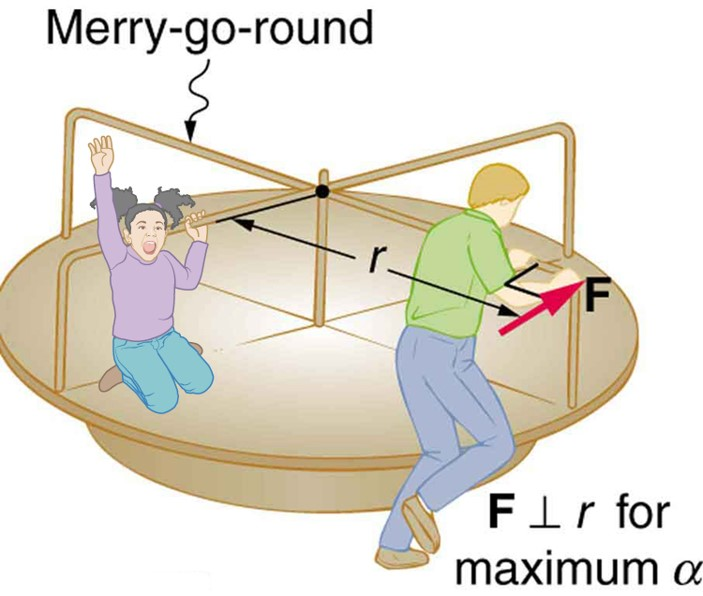
\includegraphics[width=7cm]{merrygoround.jpg}
  
  
  % {\footnotesize Image Credit: OpenStax \emph{College Physics}: 2nd Ed. Rice University. }
  
  % {\footnotesize License:} \cc\hspace{-1em}\ccby  {\footnotesize CC BY 4.0}
  
  % {\footnotesize Retrieved 2025-02-11 from \texttt{\href{https://openstax.org/books/college-physics-2e/pages/10-3-dynamics-of-rotational-motion-rotational-inertia}{https://openstax.org/books/college-physics-2e/}} }

\end{questions}

\pagebreak
%%%%%%%%%%%%%%%%%%%%%%%%%%%%%%%%%%%%%%%%

\section*{Angular Momentum}

\subsection*{Quantities}

\renewcommand{\arraystretch}{2}

\begin{tabular}{p{9em}ccp{6.5em}}
  Concept & Linear/Translational Quantity & Angular/Rotational Quantity & \hfill ``Bridge'' \\ \hline\hline
  momentum \\[1em] & units: & units:  \\\hline
\end{tabular}

\vspace{10em}

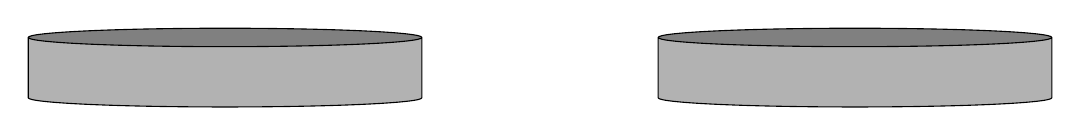
\begin{tikzpicture}
  \node[
    cylinder, 
    draw=black, 
    shape border rotate=90,
    minimum width=5cm,
    minimum height = 1cm,
    cylinder uses custom fill,
    cylinder body fill = gray!60,
    cylinder end fill = gray,
    anchor=center
    ] at (0,0) {};
  
    \node[
      cylinder, 
      draw=black, 
      shape border rotate=90,
      minimum width=5cm,
      minimum height = 1cm,
      cylinder uses custom fill,
      cylinder body fill = gray!60,
      cylinder end fill = gray,
      anchor=center
      ] at (8,0) {};
    
\end{tikzpicture}

\pagebreak

\subsection*{Practice}

\begin{questions}

\question
  An ice skater is spinning with her arms extended. She has a moment of inertia of 4.1~kg~m$^2$ and an initial angular velocity of 2.0~rad/s. She then pulls her arms in, reducing her moment of inertia to 1.5~kg~m$^2$.

  \begin{parts}
    \part 
      What is her new angular velocity after pulling her arms in?
    \part
      Calculate her initial and final rotational kinetic energy. Has her rotational kinetic energy increased or decreased? If so, explain why.
  \end{parts}
  \vs

\question
  The bicycle wheel is essentially a hoop of mass 8~kg and radius 0.4~m.  The turntable is essentially a disc of mass 5~kg and radius 0.5~m.  The instructor is essentially a particle located at the center of the axis.  If the bicycle wheel has an initial angular speed of 4.3 rad/s, what is the rate of rotation of the instructor and turntable after the wheel is flipped?
  \vs



  
\end{questions}

\end{document}